% Created 2024-06-16 Sun 00:13
% Intended LaTeX compiler: pdflatex
ocumentclass[10pt]{article}% =================================BASE====================================%
\documentclass[10pt]{report}
\usepackage[left=2cm,right=2cm,top=2cm,bottom=2cm]{geometry} % Marges
\usepackage[T1]{fontenc} % Nécessaire avec FrenchBabel
\usepackage[utf8]{inputenc} % Important pour symboles Francophones, é,à,etc
\usepackage{csquotes} % Recommandé par PDFLatex lors de la compilation. 


% Calligraphie
%\usepackage{lmodern} % Ça, ça set latin modern
%\usepackage{mathrsfs} %Permet la command \mathscr (Lettres attachées genre) \mathscr(B)

% Calligraphie
%\usepackage{pxfonts} % Met le texte ET les maths en Palatino + donne accès à des symboles math
\usepackage{palatino} % Cette commande met seulement le texte en police palatino
\usepackage{lmodern} % Pour les maths?
% Use lmodern for sans-serif
\usepackage{mathrsfs} % Permet la command \mathscr (Lettres attachées genre) \mathscr(B)





% Bibliographie
%\usepackage[backend=bibtex,style=phys,sorting=ynt]{biblatex}
\usepackage[backend=biber,sorting=ynt,style=ieee]{biblatex}
\addbibresource{/home/charlesedouard/Desktop/Travail/Documentation/master-bibliography.bib}



\usepackage{amsmath, amssymb, amsthm} % Symb. math. (Mathmode+Textmode) + Beaux théorèmes.
\usepackage{mathtools,cancel,xfrac} % Utilisation de boîtes \boxed{} + \cancelto{}{}, xfrac
\usepackage{graphicx, wrapfig} % Géstion des figures.
\usepackage{hyperref} % Permettre l'utilisation d'hyperliens.
\usepackage{color} % Permettre l'utilisation des couleurs.
\usepackage{colortbl} % Color tables
\usepackage[dvipsnames]{xcolor} % Couleurs avancées.
\usepackage{titling} % Donne accès à \theauthor, \thetitle, \thedate

% Physique
\usepackage{physics} % Meilleur package pour physicien. 


% Style
\usepackage{lipsum} % For fun
\usepackage{tikz} % Realisation de figures TIKZ.
\usepackage{empheq} % Boite autour de MULTIPLE équations
\usepackage{bbding}

% Français
\usepackage[french]{babel} % Environnements en Français.
% ==============================BASE-(END)=================================%



% ================================SETTINGS=================================%
% Pas d'indentation en début de paragraphe :
\setlength\parindent{0pt}
\setlength{\parskip}{0.15cm}

% Tableaux/tabular
% Espace vertical dans les tabular/tableaux
\renewcommand{\arraystretch}{1.2}
% Couleur des tableaux/tabular
\rowcolors{2}{violet!5}{}

% Couleurs de hyperliens :
\definecolor{mypink}{RGB}{147, 0, 255}
\hypersetup{colorlinks, 
             filecolor=mypink,
             urlcolor=mypink, 
             citecolor=mypink, 
             linkcolor=mypink, 
             anchorcolor=mypink}


\usepackage{titling} % Donne accès à \theauthor, \thetitle, \thedate

% Physique
\usepackage{physics} % Meilleur package pour physicien. 


% Style
\usepackage{lipsum} % For fun
\usepackage{tikz} % Realisation de figures TIKZ.
\usepackage{empheq} % Boite autour de MULTIPLE équations

% Français
\usepackage[french]{babel} % Environnements en Français.
% ==============================BASE-(END)=================================%





% ================================SETTINGS=================================%
% Pas d'indentation en début de paragraphe :
\setlength\parindent{0pt}
\setlength{\parskip}{0.15cm}

% Tableaux/tabular
% Espace vertical dans les tabular/tableaux
\renewcommand{\arraystretch}{1.2}
% Couleur des tableaux/tabular
\rowcolors{2}{violet!5}{}

% Couleurs de hyperliens :
\definecolor{mypink}{RGB}{147, 0, 255}
\hypersetup{colorlinks, 
             filecolor=mypink,
             urlcolor=mypink, 
             citecolor=mypink, 
             linkcolor=mypink, 
             anchorcolor=mypink}


% Numéros d'équations suivent les sections :
\numberwithin{equation}{section} 

% Les « captions » sont en italique et largeur limitée
\usepackage[textfont = it]{caption} 
\captionsetup[wrapfigure]{margin=0.5cm}

% Retirer l'écriture en gras dans la table des matières
\usepackage{tocloft}
\renewcommand{\cftsecfont}{\normalfont}
\renewcommand{\cftsecpagefont}{\normalfont}

% Change bullet style
\usepackage{pifont}
\usepackage{enumitem}
%\setlist[itemize,1]{label=\ding{224}}
\setlist[itemize,1]{label=\ding{239}}
\renewcommand{\boxtimes}{\blacksquare}
% ================================SETTINGS=================================%



% ==============================NEWCOMMANDS================================%

% Vecteurs de base :
\newcommand{\nvf}{\vb{\hat{n}}}
\newcommand{\ivf}{\vb{\hat{i}}}
\newcommand{\jvf}{\vb{\hat{j}}}
\newcommand{\kvf}{\vb{\hat{k}}}
\newcommand{\uu}{\vb{u}}
\newcommand{\vv}{\vb{v}}
\newcommand{\ust}{\vb{u}_{\ast}}

% Physics empty spaces 
\newcommand{\typical}{\vphantom{A}}
\newcommand{\tall}{\vphantom{A^{x^x}_p}}
\newcommand{\grande}{\vphantom{\frac{1}{xx}}}
\newcommand{\venti}{\vphantom{\sum_x^x}}
\newcommand{\pt}{\hspace{1pt}} % One horizontal pt space

% Moyenne numérique entre deux points de grilles. 
\newcommand{\xmean}[1]{\overline{#1}^x}
\newcommand{\ymean}[1]{\overline{#1}^y}
\newcommand{\zmean}[1]{\overline{#1}^z}
\newcommand{\xymean}[1]{\overline{#1}^{xy}}

% Tilde over psi
\newcommand{\tpsi}{\tilde{\psi}}
\newcommand{\tphi}{\tilde{\phi}}

% Nota Bene env : (\ding{89})
%\newcommand{\nb}{$\boxed{\text{\footnotesize\EightStarConvex}\pt \mathfrak{N. B.}}$\hspace{4pt}}
\newcommand{\nb}{\underline{{\footnotesize\EightStarConvex}\pt $\mathfrak{N.B.}$\vphantom{p}}\hspace{3pt}}


% Define the nota bene environment
\usepackage{tcolorbox}
\newtcolorbox{notabene}{
     colback=blue!5,
     colframe=black,
     boxrule=0.5pt,
     arc=2pt,
     left=5pt,
     right=5pt,
     top=5pt,
     bottom=5pt,
}


\newcommand{\cmark}{\ding{52}}
\newcommand{\xmark}{\ding{55}}
% ==============================NEWCOMMANDS================================%



% ==============================PAGE-TITRE=================================%
% Titlepage 
\newcommand{\mytitlepage}{
\begin{titlepage}
\begin{center}
{\Huge Contrat Été 2023 \par}
\vspace{2cm}
{\Huge \MakeUppercase{\thetitle} \par}
\vspace{2cm}
RÉALISÉ DANS LE CADRE\\ D'UN PROJET POUR \par
\vspace{2cm}
{\Huge ISMER--UQAR \par}
\vspace{2cm}
{\thedate}
\end{center}
\vfill
Rédaction \\
{\theauthor}\\
\url{charles-edouard.lizotte@uqar.ca}\\
ISMER-UQAR\\
Police d'écriture : \textbf{CMU Serif Roman}
\end{titlepage}
}
% ==============================PAGE-TITRE=================================%



% =================================ENTÊTE==================================%
\usepackage{fancyhdr}
\pagestyle{fancy}
\setlength{\headheight}{13pt}
\renewcommand{\headrulewidth}{0.025pt} % Ligne horizontale en haut

\fancyhead[R]{\textit{\thetitle}}
\fancyhead[L]{\ \thepage}
\fancyfoot[R]{\textit{\theauthor}}
\fancyfoot[L]{}
\fancyfoot[C]{} 
% =================================ENTÊTE==================================%
\author{Charles-Édouard Lizotte}
\date{23/06/2023}
\title{Carnet de bord, Université McGill}
\hypersetup{
 pdfauthor={Charles-Édouard Lizotte},
 pdftitle={Carnet de bord, Université McGill},
 pdfkeywords={},
 pdfsubject={},
 pdfcreator={Emacs 27.1 (Org mode 9.6.7)}, 
 pdflang={French}}
\begin{document}

\mytitlepage
\tableofcontents\newpage



\section{{\bfseries\sffamily DONE} Diagnostiques utiles}
\label{sec:org678c846}

Concrétement, on se souvient que les diagrammes de Hovmoller pour le modèle \emph{shallow water} résolu à l'aide du \emph{package} MUDPACK sont illustrés dans le \href{rapport-2023-06-16.org}{dernier rapport}.
Pour en avoir un avant goût, la figure \ref{fig:org7e3afe8} illustre l'état de la situation.
Essentiellement, tout se passe bien, mais des lignes horizontales viennent remettre en doute nos résultats.
Le \emph{spin up} du modèle arrive au bon moment (aux alentours de 800 jours, comme on l'observe dans le modèle résolu par transformées de Fourrier).
Ces lignes verticales sont particulièrement visible dans le rotationnel du courant. 

\begin{figure}[htbp]
\centering
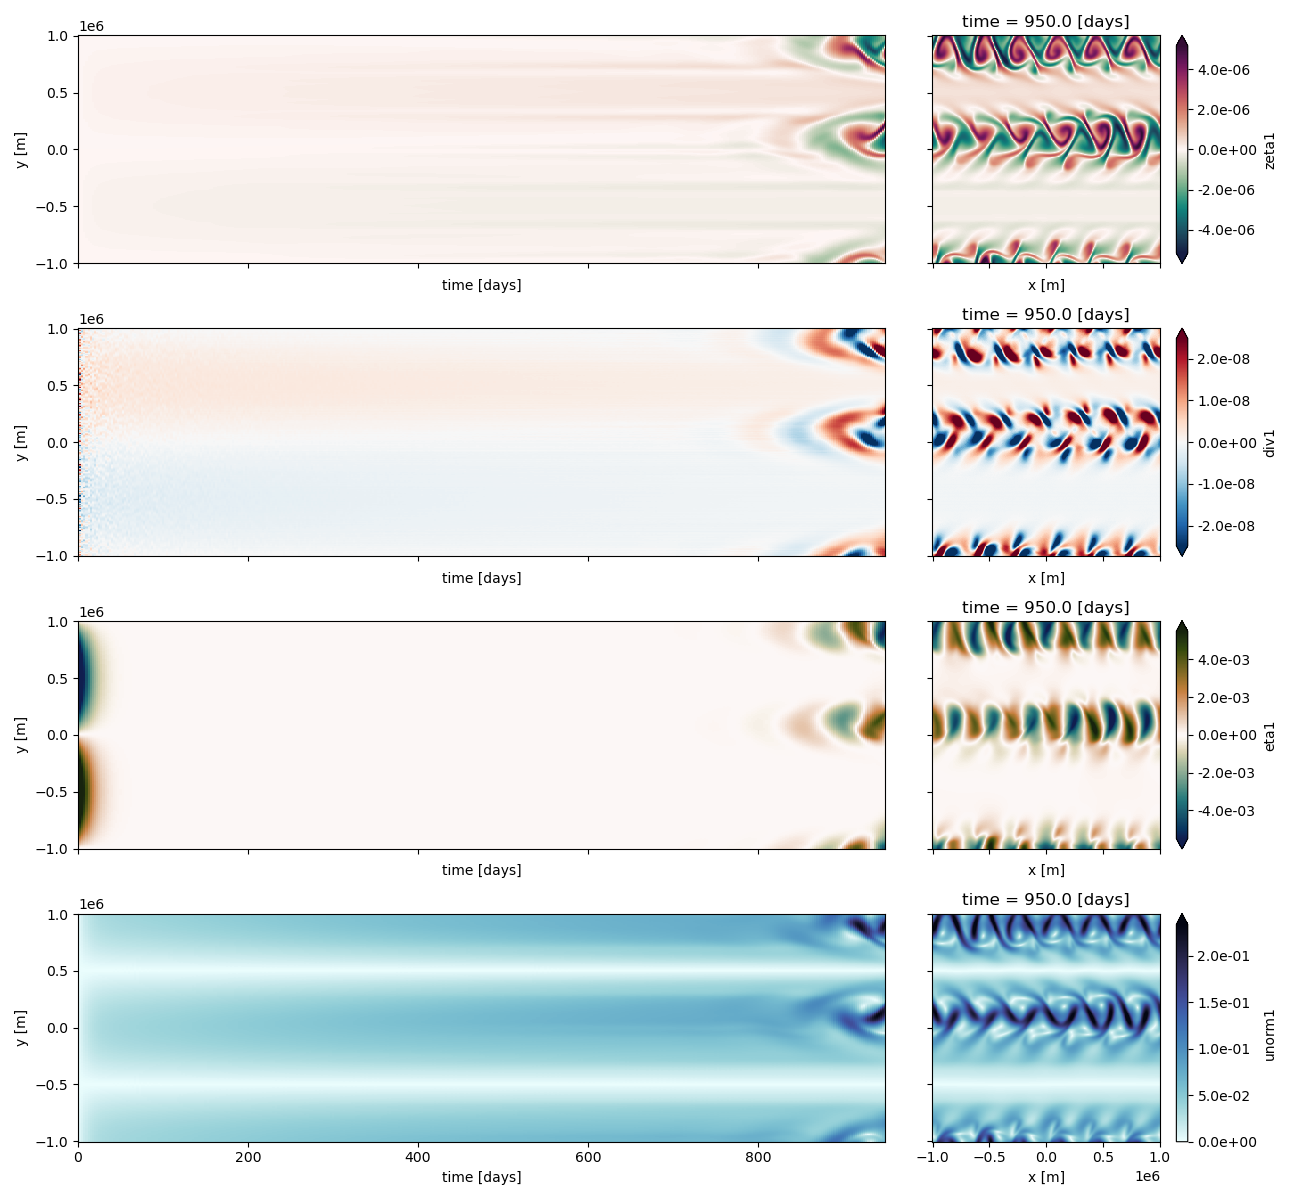
\includegraphics[width=.9\linewidth]{figures/tests/2023-06-21_hovmoller1_t=950days.png}
\caption{\label{fig:org7e3afe8}Diagrame de Hovmoller entre 0 et 950 jours pour le modèle shallow water résolu par MUDPACK. Du haut vers le bas, la vorticité, la divergence, la correction à la fonction de courant barotrope et la norme du courant. Le tout pour la première couche.}
\end{figure}



\subsection{{\bfseries\sffamily DONE} Divergence du transport barotrope (Problème réglé)}
\label{sec:orgd37b18e}
Notre première hypothèse : La solution obtenue avec MUDPACK ne se trouve pas en résolvant l'équation de la conservations de la masse, qui donnée par
\begin{equation}
\label{eq:org5b8d07f}
   \div{\uu_{BT}} = 0,
\end{equation}
mais plutôt en solvant l'équation de fonction de courant géostrophique, donnée par
\begin{equation}
   \laplacian{\psi_{BT}} = \kvf \cdot \boldsymbol{\zeta}_{BT}.
\end{equation}
Donc il faudrait vérifier que l'équation \ref{eq:org5b8d07f} (la conservation de la masse) est bel et bien respectée.\bigskip

Pour se faire, j'ai du relancer quelques \emph{runs} car -- pour sauver de l'espace sur mon poste de travail -- je ne sortais que les \emph{output} de la première couche.
Les résultats sont là :
La divergence du transport barotrope est \emph{plutôt très} nulle, ce qui veut dire que la conservation de la masse (\ref{eq:org5b8d07f}) est respectée.

\begin{figure}[!htpb]
\centering
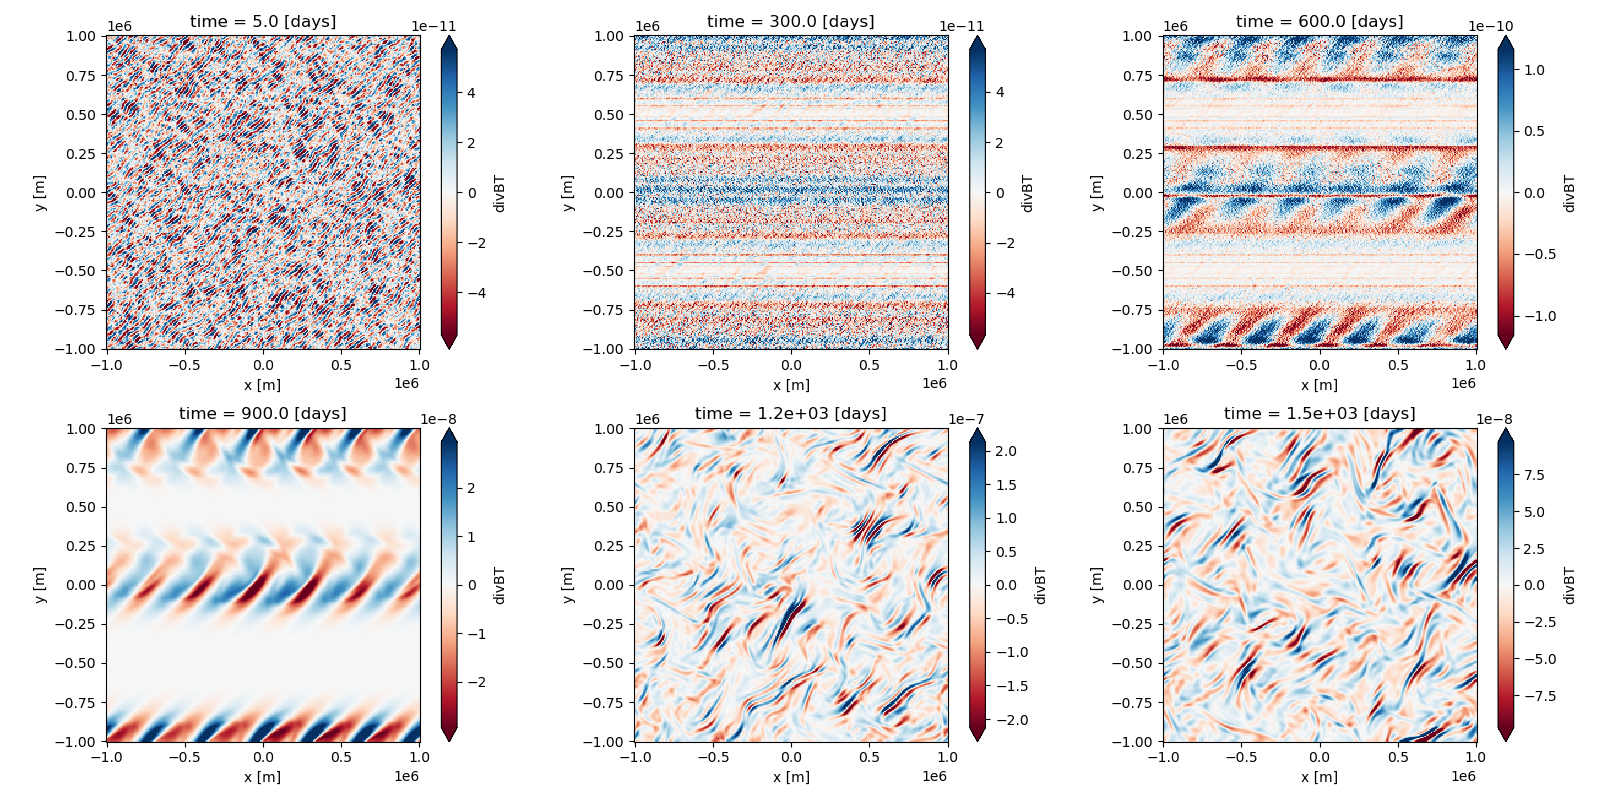
\includegraphics[width=.9\linewidth]{figures/debuggage/2023_06_21divBT1_MUD.png}
\caption{\label{fig:orged3e49c}Divergence du courant barotrope \(\qty(\div{\uu_{BT}} = \qty(1/H_{tot}) \div{\sum_i h_i \uu_i})\) à divers moments pour le modèle solvé par MUDPACK (Le temps est donnée en jours).}
\end{figure}

Lorsqu'on regarde le transport barotrope pour le modèle solvé par transformées de Fourrier, on obtient plutôt les résultats exprimés à la figure \ref{fig:org905b90c}. 

\begin{figure}[!htpb]
\centering
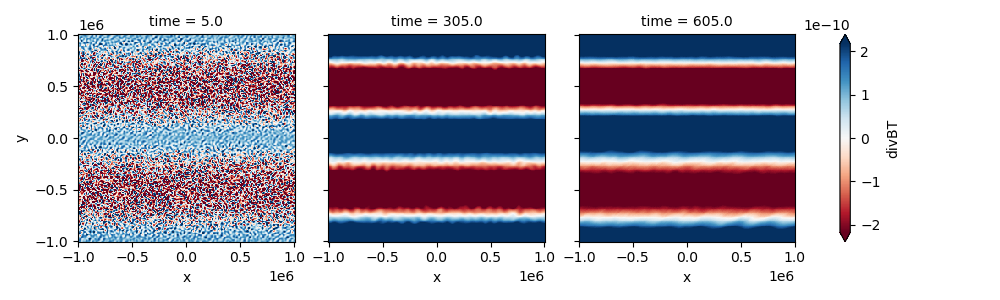
\includegraphics[width=.9\linewidth]{figures/debuggage/2023_06_21divBT1_FFT.png}
\caption{\label{fig:org905b90c}Divergence du courant barotrope  \(\qty(\div{\uu_{BT}} = \qty(1/H_{tot}) \div{\sum_i h_i \uu_i})\) à divers moments pour le modèle solvé par FFTW (Le temps est donnée en jours).}
\end{figure}

Normalement, ça devrait être complétement nul, ce qui est quand même inquiétant.
J'ai passé une bonne journée à tenter de débugger tout ça, mais sans succès, malheureusement.
Je tient à metionner que les dérivées de chaque côté sont quand même très semblables.
Par exemple, comme illustré à la figure \ref{fig:orgaa16c1b}, les dérivées sont pratiquement identiques, mais de petits écarts se sont creusée quand on les additionne pour obtenir la divergence. 

\begin{figure}[!htpb]
\centering
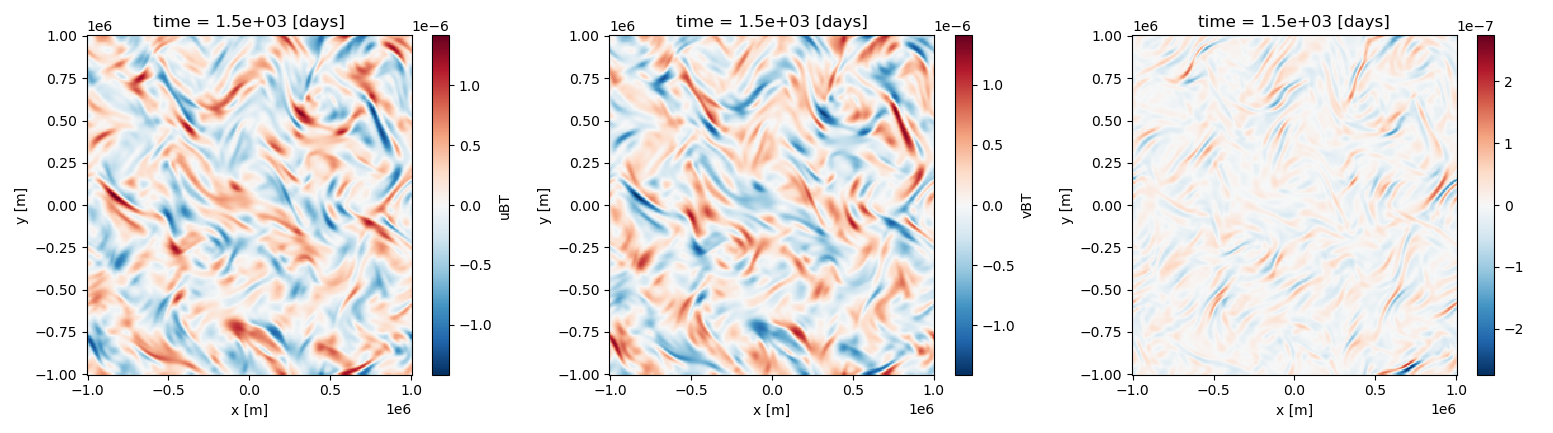
\includegraphics[width=.9\linewidth]{figures/debuggage/2023_06_27_comp_divBT.png}
\caption{\label{fig:orgaa16c1b}Dérivées horizontales et verticales du courant barotrope et leur addition (la divergence), à droite.}
\end{figure}

Il est difficile à dire d'où vient cette erreur.
Personellement, je pense que ça vient du fait qu'on fait rouler notre modèle en 512, mais que les output sont en 256.
Lorsqu'il y a des changement abruptes et comme notre résolution n'est pas excelente, on pourrait voir des artefacts qui s'apparentent à ce genre d'erreurs.
Comme on voyait aussi ça avec le modèle \emph{shallow water} FFTW, je ne m'inquiéterais pas trop, mais ça serait pertinent de le mentionner à David ou Louis-Philippe.
En gros, ma théorie c'est que la résolution est pas suffisante pour qu'on ait un aperçu réel de ce que la vraie grille nous donne.


\subsection{{\bfseries\sffamily DONE} C'est réglé! L'erreur est bel et bien dans mon code}
\label{sec:orgef594e7}
OK. C'est confirmé, l'erreur vient de mon code.
En effet, lorsqu'on fait des opérations sur les \emph{outputs} -- particulièrement lorsqu'on applique des dérivées -- il faut avoir une résolution exacte et non un sous-échantillon des résultats réels.
Pour l'exprimer, voir l'illustration suivante (figure \ref{org66062a5}). \bigskip

\begin{figure}[h!]
\begin{center}
\begin{tikzpicture}
%
\draw [dotted,thin,gray] (0,0) grid (3,3);
\draw [thin, red ,dashed](-0.1,-0.1) rectangle (2.20,1.1);
\draw [thin, blue,dashed](-0.15,-0.15) rectangle (1.1,2.20);
%
\foreach \i in {0,2}
{\foreach \j in {0,2}
{\draw [thick, red!50] (\i,\j+1) -- (\i,\j) ;
 \draw [thick,blue!50] (\i,\j) -- (\i+1,\j) ;}}
%
\foreach \i in {0,2}
{\foreach \j in {0,2}
{\draw [-latex,thin,red!50 ] (\i,0.5+\j) -- (\i+0.15,0.5+\j);
 \draw [-latex, thin,blue!50] (0.5+\i,\j) -- (0.5+\i,\j+0.15);}}
%
\foreach \i in {0,1,2,3}
\foreach \j in {0,1,2,3}
{{\filldraw [black!85] (\i,\j) circle (0.8pt);}}
%
\draw (7,1.5) node [rectangle, draw=black,fill=white] {\hspace{0.3cm}$\div{\uu} = \color{blue!70}\qty(\pdv{u}{x}) \color{black} + \color{red!70} \qty(\pdv{v}{y})\hspace{0.3cm}\venti$};
\end{tikzpicture}
\end{center}
\caption{\label{org66062a5}Illustration de l'erreur engendrée par le sous-échantillonnage des données réelles. Le résultat donne des lignes diagonales croissantes qui apparaissent un peu partout sur le domaine.}
\end{figure}

Par conséquent, on doit oublier toute forme de dérivées dans nos calculs à partir de maintenant.
C'est d'ailleurs un problème que j'ai eu lors de ma maîtrise sans en être conscient.
Je suis quand même fier que ça soit réglé.
Par contre, ça signifie que beaucoup de transformées de Fourrier ont des résultats douteux dans mon mémoire de maîtrise.
Louis-Philippe, si tu lis ce texte, j'espère que tu vas empêcher tes prochains étudiant-es de faire ça et me pardonner d'avoir péché. \bigskip

\subsection{Nouvelle run avec la divergence barotrope comme output dans le modèle}
\label{sec:org6bd6208}

Comme je m'y attendais, le résultat est complétement différent lorsqu'on sort en \emph{output} la divergence du courant barotrope.
Malheureusement, il semble toujours y avoir quelque chose qui cloche.
Les lignes horizontales persistent dans le modèle résolu par \emph{MUDPACK}.

\begin{figure}[!htpb]
\centering
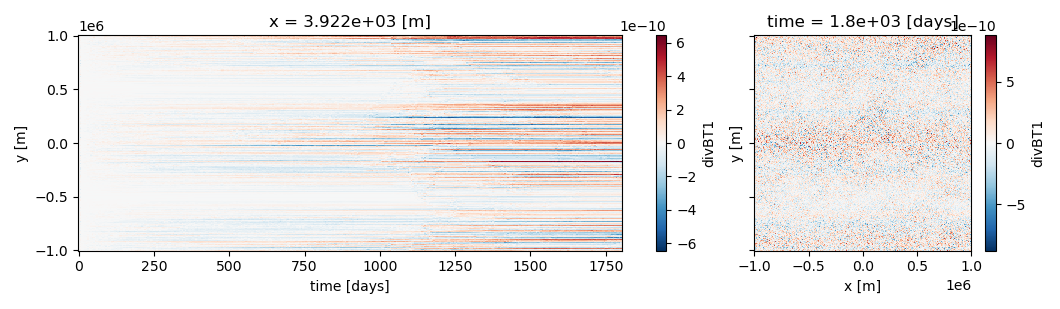
\includegraphics[width=.9\linewidth]{figures/debuggage/2023_07_03_comp_divBT.png}
\caption{\label{fig:orge972714}Divergence du courant barotrope avec le dernier test de MUDPACK.}
\end{figure}





\section{{\bfseries\sffamily DONE} Problème conceptuel avec MUDPACK (Vrai ou faux?)}
\label{sec:org42a7830}

\subsection{Confirmation sur la périodicité de la frontière avec MUDPACK}
\label{sec:org1a5602f}

\begin{figure}[!htpb]
\centering
\includegraphics[width=.9\linewidth]{figures/MUDPACK/test_sans_frontière.png}
\caption{\label{fig:org3cd95ca}Test de MUDPACK où le dernier point n'est pas inclu comme un point périodique.}
\end{figure}

Je confirme à 100 \% qu'il faut inclure la frontière aux deux extrémités dans \emph{MUDPACK} lorsqu'on donne une frontière périodique.
C'est relativement simple à tester, mais lorsqu'on le fait, on voit apparaître des erreurs significatives.
Par exemple, si l'on regarde à la figure \ref{fig:org3cd95ca}, on note une erreur d'environ 0.6\% sur la solution, soit une erreur deux fois plus grande qu'avec l'autre test.
Je pense qu'il est aussi intéressant de mentionner qu'on voit apparaître des lignes verticales dans la solution calculée par \emph{MUDPACK}, ce qui pourrait être analogue au problème que nous avons dans notre propre modèle numérique. 
Tandis que lorsqu'on regarde la figure \ref{fig:org294c50a}, on note une erreur de 0.012\% sur la solution.
L'erreur prend plus la forme d'une erreur numérique diffuse sur le domaine.
Contrairement à l'autre figure, on note aussi que cette erreur est loin des bords. \bigskip

\begin{figure}[!htpb]
\centering
\includegraphics[width=.9\linewidth]{figures/MUDPACK/test_avec_frontière.png}
\caption{\label{fig:org294c50a}Test de MUDPACK où le dernier point est inclu comme un point périodique, de sorte que phi(1)=phi(nx).}
\end{figure}

Au regard de ces résultats, je confirme -- hors de tout doute -- qu'il faut inclure la frontière dans le cas périodique.
Pour le tester, comme on trouve la solution entre les points 1 et 5, on change tout simplement la définition du paramètre \(dx\) pour obtenir une solution réelle qui représente bien les deux cas.
Comme, le paramètre \(dx\) entre dans la définition de la solution réelle, on joue un tour à \emph{MUDPACK} pour inclure ou non la frontière, comme illustré dans la figure \ref{org15d1dec}. \bigskip

\begin{figure}[!h]
\begin{center}
\begin{tikzpicture}
\draw (0.5,0.75) node [] {a)};
% >> Dotted lines :
\foreach \i\j in {1/-1, 2/-0.524, 3/-0.706, 4/-1.294, 5/-1.476, 6/-1}
{
\draw[dotted] (\i,0) -- (\i,\j);
}
% >> balls : 
\draw [] (1,0) -- (6,0);
\foreach \i in {1,...,5}
{
\filldraw [black,fill=Violet!20]  (\i,0) circle (6pt) node [] {$\mathrm{\i}$};
}
\filldraw [black,fill=white]  (6,0) circle (6pt) node [] {6};
\draw (1,-1) sin (2.25,-0.5) cos (3.5,-1) sin (4.75,-1.5) cos (6,-1);
% >> Text :
\draw (2.2,-1.25) node {$n_x = 5$};
\draw (2.2,-1.75) node {$dx = L_x/n_x$};
% >> Domain line 
\node [] at (3.0,0.75) (domain) {Domaine MUDPACK} ;
\draw [|-] (1,0.75) -- (domain);
\draw [-|] (domain) -- (5,0.75);
\end{tikzpicture}
% END
\hspace{2cm}
% BEGIN
\begin{tikzpicture}
\draw (0.5,0.75) node [] {b)};
\draw [] (1,0) -- (5,0);
\foreach \i\j in {1/-1, 2/-0.5, 3/-1, 4/-1.5, 5/-1}
{
\draw[dotted] (\i,0) -- (\i,\j);
}
\foreach \i in {1,...,5}
{
\filldraw [black,fill=Violet!20]  (\i,0) circle (6pt) node [] {\i};
}
\draw (1,-1) sin (2,-0.5) cos (3,-1) sin (4,-1.5) cos (5,-1);
% Text
\draw (2.0,-1.25) node {$n_x = 5$};
\draw (2.2,-1.75) node {$dx = L_x/(n_x-1)$};
% Domain line
\node [] at (3.0,0.75) (domain) {Domaine MUDPACK} ;
\draw [|-] (1,0.75) -- (domain);
\draw [-|] (domain) -- (5,0.75);
\end{tikzpicture}
\end{center}
\caption{\label{org15d1dec}Illustration des shéma numériques pour le test avec MUDPACK. a) Solution plus grande que le domaine compilé -- les points 1 et 6 sont périodiques. b) Solution couvre le domaine --  les points 1 et 5 sont périodiques. Dans les deux cas, on compile un domaine contenant \(n_x\) points dans le solveur MUDPACK.}
\end{figure}


\section{MUDPACK avec une grille de base plus large}
\label{sec:org1599612}
J'ai relancé le modèle avec un \emph{nx} de 640 points, ce qui me permet de mettre la plus petite grille de \emph{MUDPACK} à 5 points de large.
Considérant la nature périodique de la solution qu'on cherche, 5 points devraient être suffisants pour représenter la solution à la plus petite échelle -- en opposition à 2 points.
Dans la documentation, il était suggéré de prendre 2, 3 ou 5 et de se retenir de prendre de plus grandes grilles.
Malheureusement, le résultat sur les diagrammes de Hovmoler était le même, comme on peut le voir à la figure \ref{fig:org97821c4}.


\begin{figure}[!htpb]
\centering
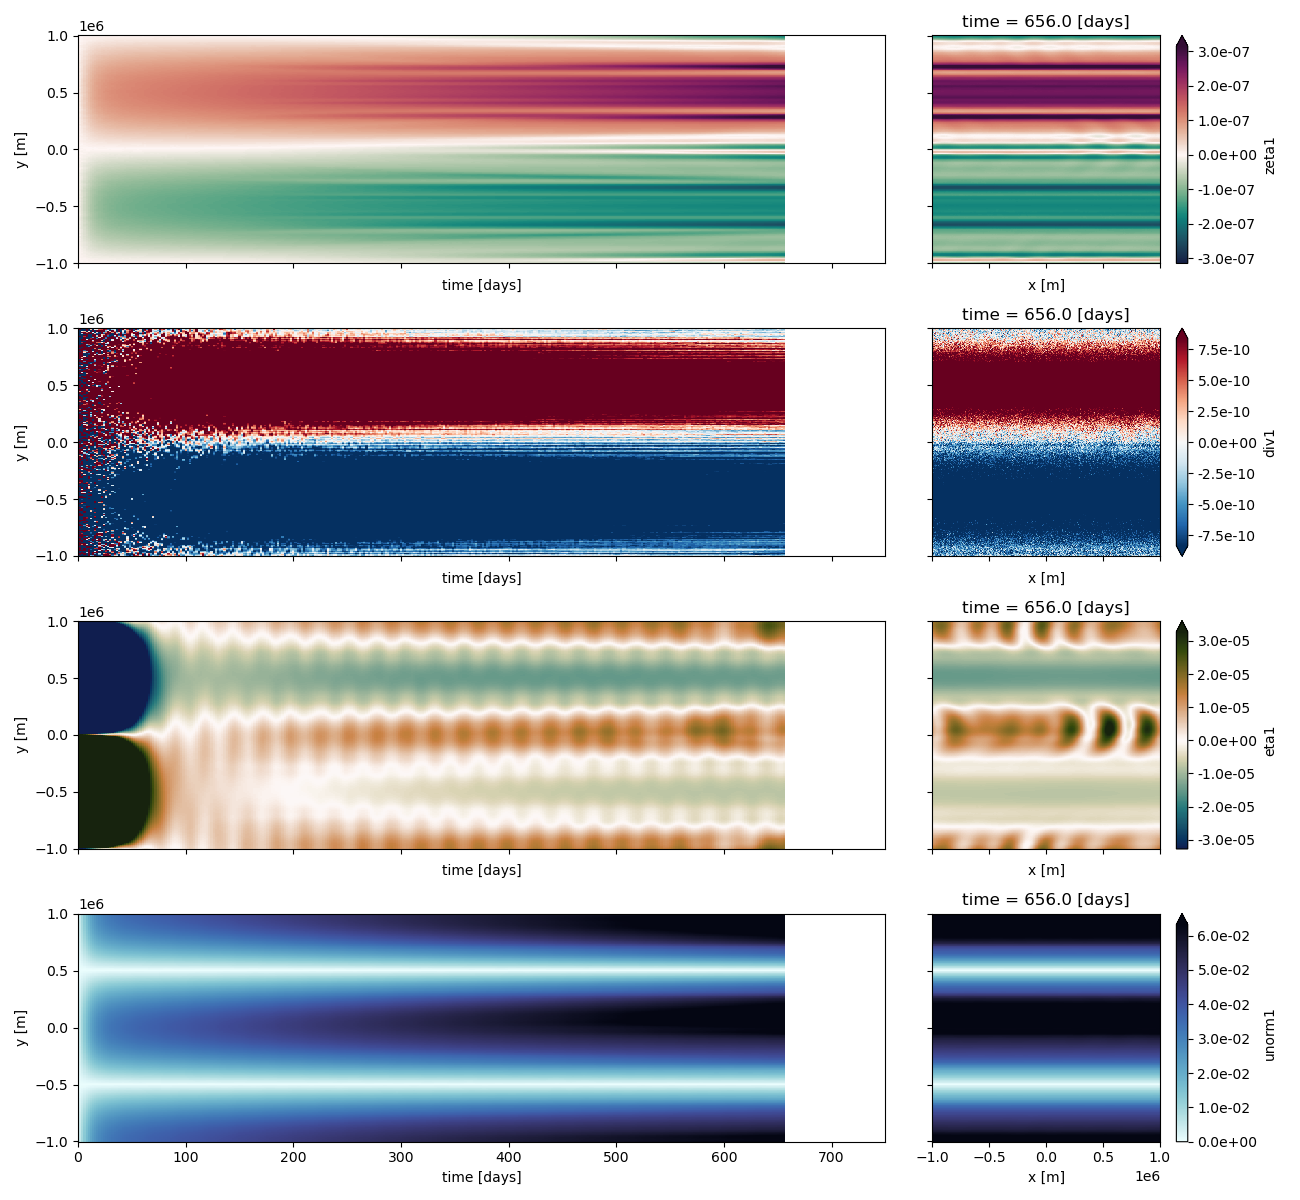
\includegraphics[width=.9\linewidth]{figures/tests/2023-06-28_hovmoller1_nx640_t=750days.png}
\caption{\label{fig:org97821c4}Diagramme de Hovmoller pour la première couche avec un nx de 640 points.}
\end{figure}
\end{document}